\documentclass[10pt]{article}
\usepackage[margin=0.82in]{geometry}
\usepackage[T1]{fontenc}
\usepackage{lmodern,microtype,amsmath,amssymb,booktabs,longtable,array,graphicx,xcolor}
\usepackage[numbers,sort&compress]{natbib}
\usepackage[colorlinks=true,linkcolor=blue!45!black,citecolor=blue!45!black,urlcolor=blue!45!black]{hyperref}
\usepackage{placeins}
\setlength{\parskip}{3pt}
\setlength{\parindent}{1em}
\setlength{\tabcolsep}{4pt}
\renewcommand{\arraystretch}{1.12}
\newcommand{\SocialLean}{0.644}
\newcommand{\SocialVsText}{0.111}
\newcommand{\CautionLean}{0.867}
\newcommand{\CautionVsText}{0.389}
\newcommand{\ExploreLean}{0.467}
\newcommand{\ExploreVsText}{0.333}
\newcommand{\AvoidedPct}{83.5}
\newcommand{\CautionAgreePct}{99.0}
\newcommand{\SocialAgreePct}{98.1}
\newcommand{\PostCuts}{167}
\newcommand{\ResolvedCuts}{130}
\newcommand{\CensoredCuts}{37}
\newcommand{\MaxDelay}{12}
\newcommand{\ResolvedDelay}{1.44}
\newcommand{\SlowCuts}{33}
\newcommand{\DecodeSeconds}{0.453}
\newcommand{\EvidenceFiles}{232}
\newcommand{\AuditedImageRecords}{143}
\newcommand{\ScalarChecks}{22490}

\title{The Lookout and the Captain:\\
Mode Conditioning and Event-Triggered Decoding\\in Frozen Vision-Language Models}
\author{Franci Penov\\Kortexa AI\\\texttt{francip@kortexa.ai}}
\date{September 7, 2026}
\begin{document}
\maketitle
\begin{abstract}
A small vision model can select a behavioral mode for a larger model and
decide when that model should run. We study these two functions separately
in frozen vision-language models with nominal sizes of 450M, 3B, and 27B
parameters. A learned 256-dimensional packet encodes an operator's mode
instruction. State-conditioned receivers inject the packet into three
language-model layers; the larger model also receives the image. The task
has three possible actions: greet, stop, and proceed. On held-out photographs,
the packet changes action selection, with substantial variation across
modes and adapter seeds. At 27B, its increase over a constant adapter is
\SocialLean{}, \CautionLean{}, and \ExploreLean{} for the three modes.
Detector-controlled packet selection incurs errors that can be traced to
the selected packet on each image. In a replay of short image streams,
waking the model on changes in the detector's verdict avoids \AvoidedPct{}\%
of model calls, with \SocialAgreePct{}\% social-mode and
\CautionAgreePct{}\% caution-mode agreement with decoding every frame at
27B. This is an invocation result, not a measured energy saving or a delay
guarantee. Rendered-scene tests expose failures that depend on the adapter
seed, instruction phrase, training domain, and constant-adapter baseline.
The results support mode conditioning and selective invocation in this
restricted task. They do not establish general instruction robustness,
robot-control safety, or transfer across arbitrary visual domains.
\end{abstract}

\section{Introduction}
An image can determine both what a model should do and whether it needs
to run again. These are different decisions. A person detector can report
that someone is present without determining whether a robot should greet
that person or stop. An operator supplies that policy. Similarly, a change
in pixels need not require a new action, while a small change that alters
the task state may require one.

We examine a two-model arrangement. The \emph{lookout} is a small person
classifier or detector. The \emph{captain} is a frozen vision-language model
that receives the camera image and produces an action. An external policy
maps the detector's binary verdict to a mode packet: use the operator's
social or caution mode when a person is detected, and explore mode
otherwise. A second rule decides whether to invoke the captain or retain
its previous action. The packet represents a mode instruction. In the
main experiments it does not encode the detector's visual features or
describe an object.

This construction lets us ask four empirical questions. Does the packet
change action selection beyond a separately trained constant adapter?
How do detector errors change that effect? How does conditioning behave
under contrary text, missing images, and a new rendering domain? Finally,
how often can the model reuse an action while matching a model invoked
on every frame?

The evidence is a controlled case study, not a general robot benchmark.
We use three frozen hosts, three adapter seeds for the main comparisons,
fixed photographic evaluation sets, and matched interventions on each
image. The larger host demonstrates that the mechanism operates beyond a
small language model. The two model families differ in architecture and
pretraining, so their comparison is not a controlled scaling law.
Negative results are part of the answer: some modes barely improve over
the constant adapter, some held-out instruction phrases fail, and mixed
visual-domain training does not give a uniformly better adapter.

\section{Relation to existing methods}
Prefix tuning learns continuous activations that guide a frozen language
model \citep{li2021prefix}. Activation engineering constructs steering
directions from activation differences between prompts
\citep{turner2024steering}, while representation engineering studies
control and monitoring through model representations \citep{zou2023rep}.
Our packet and receivers are trained components, and each receiver reads
the target model's current residual state. This differs from adding a
single fixed steering direction, but does not make the broader idea of
activation-based conditioning new.

Hypernetworks generate the weights of another network
\citep{ha2016hypernetworks}. The implementation here instead generates a
latent packet and residual updates; it does not generate LoRA matrices
or alter the host's stored weights. We therefore describe the actual
emitter and receivers rather than treating all conditional modules as
the same architecture.

Selective invocation also differs from speculative decoding
\citep{leviathan2023fast}. Speculative decoding uses a smaller model to
propose tokens that a larger model verifies. Here the detector decides
whether to skip a whole model invocation and retain the last action.
There is no token-level verification or exact output-distribution
guarantee. Our contribution is the combined experimental analysis of
these mode-selection and invocation decisions, including controls that
locate their failures.

\section{Method}
\subsection{Task, hosts, and photographic data}
The model answers a fixed request for a JSON object whose action is
\texttt{greet}, \texttt{stop}, or \texttt{proceed}. The reference policy is:
social mode greets a present person; caution mode stops for a present
person; explore mode always proceeds; every mode proceeds on an absent
image. These are task labels, not executable robot actions.

The hosts are LiquidAI/LFM2.5-VL-450M, LiquidAI/LFM2.5-VL-3B, and
Qwen/Qwen3.8-27B \citep{liquid450,liquid3b,qwen27}. Their measured language
towers have 16, 30, and 64 layers, with hidden widths 1024, 2048, and
5120. All host parameters are frozen. CUDA runs use bfloat16 host
computation and float32 adapter computation. Qwen's thinking mode is
disabled. Model identifiers, available revision pins, and checkpoint
hashes accompany the code.

We draw photographs from COCO val2017 \citep{lin2014coco}. A present
image has at least one non-crowd person annotation whose
\texttt{area}/image-area is at least 0.05. This uses the annotation's
area, not its bounding-box area; the historical source labels that field
imprecisely. An absent image has no person annotation. Other images are
excluded. The eligible pools contain 1505 present and 2307 absent images.
Sampling uses sorted image IDs and a fixed Python random seed of 42.

The adapter training set contains 40 present and 40 absent photographs.
The initial evaluation set contains a disjoint 30 present and 30 absent
photographs. Detector-switch and box experiments use a further disjoint
100 present and 100 absent photographs. The remaining 3472 eligible
photographs train the small classifier and provide detector-size
calibration. Each evaluation set is shared across host and adapter
seeds. Reusing it for subsequent design choices makes the follow-ups
exploratory evaluations on a reused set, rather than new independent
confirmation. COCO val2017 is also a standard detector validation set;
this study cannot establish that it is unseen by the pretrained hosts.

\subsection{A packet and three state-conditioned receivers}
There are ten instruction phrasings per mode. Positions 0--7 train the
adapter; positions 8 and 9 are held out. For each phrase, we run a
text-only exchange containing the mode assignment and an assistant
acknowledgment, and extract the last-position hidden state at layer
$\operatorname{round}(0.79L)$. The packet source therefore contains the
mode text, not image features.

Let $s$ be that source state. A mean and scalar scale fitted on the
24 training-phrase states center and normalize $s$, followed by RMS
normalization. The emitter is a linear map and GELU:
\begin{equation}
 z=\operatorname{GELU}(W_E\,\operatorname{RMSNorm}((s-\mu)/\sigma)+b_E),
 \qquad z\in\mathbb{R}^{256}.
\end{equation}
At each injection layer $\ell$, the receiver combines projections of
$z$, the RMS-normalized current residual $h_{\ell,t}$, and a learned
position embedding $e_t$. Packet and residual projections each have
width 128, and the position embedding has width 64. A 320-to-512-to-$d$
MLP with GELU produces $u_{\ell,t}$, where $d$ is the host width.
The receiver reads a detached residual state; training still propagates
through the frozen host operations to the adapter.
\begin{equation}
 h'_{\ell,t}=h_{\ell,t}
   +\alpha\lVert h_{\ell,t}\rVert_2
       \frac{u_{\ell,t}}{\max(\lVert u_{\ell,t}\rVert_2,10^{-6})}.
\end{equation}
The three injection layers are the rounded depth fractions
$(0.29,0.46,0.63)$, clamped to valid layers and deduplicated. The resulting
indices are $(5,7,10)$, $(9,14,19)$, and $(19,29,40)$; source indices
are 13, 24, and 51. These indices were not selected by a layer sweep.
Injection begins at the last prompt position and continues during
decoding. There are 16 learned position embeddings, and later positions
use the last embedding. The operating dose is $\alpha=0.15$.

The receivers have separate parameters at each layer and share the
packet. Because they read image-conditioned host states, a packet that
is independent of the image can still produce an image-dependent
intervention. Its text-only source does not imply domain-independent
behavior.

The emitter and three receivers contain approximately 2.83M, 5.06M,
and 11.75M trainable parameters for the respective hosts, excluding
the 771-parameter auxiliary training head. The packet width remains
256 while the receiver output width follows the host. This parameter
count describes the complete emitter and receiver bank.

\subsection{Training and comparison arms}
We train each adapter for 192 optimizer steps with eight sequentially
accumulated examples per step, AdamW at learning rate 0.003, no weight
decay, and adapter gradient-norm clipping at 1.0. Each example draws a
mode, a training image, and, for the mode adapter, a training phrase.
The loss is teacher-forced cross entropy on the reference JSON action
and EOS token. A three-class auxiliary head on the mode packet adds a
cross-entropy term of weight one. The head is trained but not used at
evaluation. Its parameters are optimized alongside the adapter; the
historical clipping call covers the adapter parameters only.

A separate \emph{constant adapter} uses the mean training source state
for every mode and has no auxiliary mode head. Its image-to-action
training targets still span the three modes. It is therefore a learned
baseline with its own action preferences, not the unmodified frozen
model. The mode and constant adapters also consume different random
draws in training. The comparison measures the effect of the complete
trained conditioning arrangement; it does not isolate the auxiliary
loss or equalize every training choice.

The four main arms are:
\begin{itemize}
\item \textbf{Packet:} the mode adapter receives the requested mode
packet; the prompt contains no mode instruction.
\item \textbf{Swapped:} the same adapter receives the next mode in a
fixed social--caution--explore cycle. This is a deterministic wrong-mode
control, called \texttt{shuffled} in the saved records.
\item \textbf{Constant:} the constant adapter receives its fixed source;
the prompt contains no mode instruction.
\item \textbf{Text:} the constant adapter remains active and the prompt
contains the requested mode instruction.
\end{itemize}
Thus Packet versus Text compares two trained adapter arrangements.
It does not compare packet conditioning with an untouched model's
best possible prompt. There is no broad prompt search.

The main seeds are 42, 1042, and 2042. Before evaluation, recorded checks
require unchanged sampled host parameters, identical next-token logits
at zero injection dose on a test image, and at least 0.90 teacher-forced
token accuracy on the held-out phrases with eight training images.
All main adapter pairs pass. The parameter check samples parameters,
and the phrase check includes predictable JSON syntax; neither is a
complete weight-integrity or held-out action-accuracy test.

\subsection{Evaluation and uncertainty}
Decoding is greedy with a maximum of 24 new tokens. The parser selects
the first valid JSON object containing an allowed action, otherwise
the first allowed action word, and otherwise \texttt{other}. We replay
this parser on every saved individual-image response in the audit.
Stream records retain the action and parse path, rather than the full
generated response.

For mode $m$, let $p_A(m)$ be the fraction of present images on which
arm $A$ returns the mode's target action. We report the raw shares and
paired differences, especially $p_{\rm Packet}-p_{\rm Constant}$.
On absent images, greet or stop is a task error; proceed is correct.
A high agreement with another model is reported separately from
reference-policy correctness.

Means give each tested adapter seed equal weight. Intervals are
post-hoc, pointwise 95\% percentile bootstrap intervals with 10,000
replicates. We resample image IDs within a label, retaining all paired
arms and the tested seeds for each image. For rendered data, a
within-label observation is one scene draw. For streams, we resample
complete 16-step episodes. We do not treat repeated seeds, arms, or
frames in an episode as independent observations.

These intervals describe sampling variation conditional on the tested
seeds, fixed phrase assignment, and source population. They do not
cover an unseen seed distribution, new instruction phrasings, or
adaptive experiment selection. We also give per-seed results. At a
boundary, percentile intervals can collapse to a point; an empirical
zero error with such an interval does not prove zero population error.
The historical plan contains dated questions, thresholds, amendments,
and readings. Those internal records document the exploratory sequence;
they are not an external preregistration, and their reading bands are
not statistical significance tests.

\section{Conditioning on photographs}
Table~\ref{tab:conditioning} and Figure~\ref{fig:conditioning} show clear
mode-dependent effects, but no uniform benefit in every host and mode.
Caution improves substantially on all three hosts. Social mode on 3B
has a mean improvement of only 0.022, and explore mode on 450M improves
by 0.044. Both intervals include zero. At 27B, Packet exceeds Text
by \SocialVsText{}, \CautionVsText{}, and \ExploreVsText{} for social,
caution, and explore respectively, under the particular Text control
defined above.

\begin{table}[htbp]\centering\small
\caption{Target-action share on 30 present photographs, averaged over
three adapter seeds. Brackets give paired image-bootstrap intervals.
Constant is the separately trained constant adapter.}\label{tab:conditioning}
\begin{tabular}{llrrrll}\toprule
Host & Mode & Constant & Packet & Text & Packet--Constant & Packet--Text\\\midrule
450M & Social & 0.300 & 0.633 & 0.967 & 0.333 [0.144, 0.511] & -0.333 [-0.489, -0.178] \\
450M & Caution & 0.222 & 1.000 & 0.922 & 0.778 [0.700, 0.856] & 0.078 [0.033, 0.133] \\
450M & Explore & 0.478 & 0.522 & 0.533 & 0.044 [-0.089, 0.178] & -0.011 [-0.144, 0.122] \\
3B & Social & 0.467 & 0.489 & 0.922 & 0.022 [-0.211, 0.256] & -0.433 [-0.600, -0.256] \\
3B & Caution & 0.089 & 0.756 & 0.911 & 0.667 [0.567, 0.756] & -0.156 [-0.256, -0.033] \\
3B & Explore & 0.444 & 1.000 & 0.967 & 0.556 [0.433, 0.678] & 0.033 [0.000, 0.078] \\
27B & Social & 0.333 & 0.978 & 0.867 & 0.644 [0.567, 0.722] & 0.111 [0.011, 0.222] \\
27B & Caution & 0.133 & 1.000 & 0.611 & 0.867 [0.789, 0.933] & 0.389 [0.289, 0.489] \\
27B & Explore & 0.533 & 1.000 & 0.667 & 0.467 [0.389, 0.533] & 0.333 [0.256, 0.411] \\

\bottomrule\end{tabular}
\end{table}

\begin{figure}[htbp]\centering
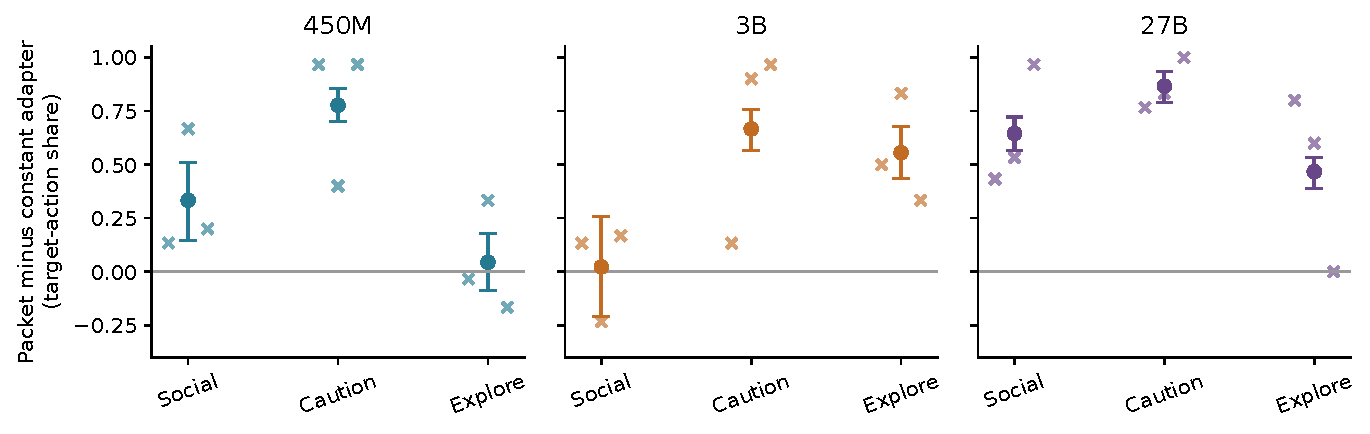
\includegraphics[width=.96\linewidth]{conditioning.pdf}
\caption{Conditioning effects on present photographs. Circles and error
bars show means and image-bootstrap intervals conditional on the three
seeds; crosses show the three separate seed means.}\label{fig:conditioning}
\end{figure}

Wrong-mode packets change the actions, including when Packet and
Constant have similar means. This is evidence that packet content
matters, although its effect can be poorly aligned with the requested
task. Absent-image behavior must be examined separately:
27B Packet never greets in social mode on the 30 absent photographs,
but its mean caution stop share is 0.044. Table~\ref{tab:controls}
reports both the wrong-mode contrast and absent-image shares.
The findings establish restricted action conditioning rather than
general multimodal generation or reliable obstacle avoidance.

\section{Replacing the annotation with a detector}
\subsection{Detector selection and measured error}
The external switch chooses the requested social or caution packet
when its input verdict is present, and the explore packet otherwise.
An oracle switch uses the COCO label. A learned classifier uses
ImageNet-pretrained MobileNetV3-small features \citep{howard2019mobilenet}
with a two-class linear head trained for three epochs, seed 42, on
the 3472-image remainder. An off-the-shelf YOLO26 detector
\citep{ultralytics2026} uses a person box with confidence at least 0.25
and bounding-box fraction at least 0.05 as its present rule.
The box rule and COCO annotation-area rule are not identical.

Table~\ref{tab:detectors} gives the detector results. Detector size was
chosen by the fewest misses on the separate calibration remainder,
breaking ties toward the smaller detector. The medium detector has
the fewest calibration misses. Both small and medium detectors have
zero misses on the 100 present evaluation photographs, but still have
false alarms. This is a finite-set observation, not proof of a
perfect detector.

\begin{table}[htbp]\centering\small
\caption{YOLO26 detection results. Evaluation has 100 present and 100
absent images; calibration has 1335 present and 2137 absent images.
Timing is the recorded batch-inference wall time per calibration
image, including the prototype's processing overhead.}\label{tab:detectors}
\begin{tabular}{lrrrrrr}\toprule
Detector & Params (M) & Eval misses & Eval false alarms &
Calib.\ misses & Calib.\ false alarms & ms/image\\\midrule
YOLO26N & 2.41 & 5 & 2 & 25 & 25 & 3.49 \\
YOLO26S & 9.50 & 0 & 1 & 12 & 22 & 3.58 \\
YOLO26M & 20.41 & 0 & 2 & 10 & 22 & 4.43 \\

\bottomrule\end{tabular}
\end{table}

\begin{table}[htbp]\centering\small
\caption{Detector minus oracle target-action share on the 100 present
evaluation images, with paired intervals across images and means over
three seeds. Small and medium YOLO host runs were completed on the two
LFM hosts; 27B uses the nano detector.}\label{tab:switch}
\begin{tabular}{llll}\toprule
Host & Detector & Social gap & Caution gap\\\midrule
450M & MobileNet & -0.053 [-0.093, -0.020] & -0.077 [-0.127, -0.033] \\
3B & MobileNet & -0.037 [-0.077, -0.007] & -0.073 [-0.117, -0.037] \\
450M & YOLO26n & -0.027 [-0.060, 0.000] & -0.037 [-0.073, -0.007] \\
3B & YOLO26n & -0.013 [-0.033, 0.000] & -0.033 [-0.067, -0.007] \\
27B & YOLO26n & -0.033 [-0.070, -0.007] & -0.047 [-0.090, -0.010] \\
450M & YOLO26s & 0.000 [0.000, 0.000] & 0.000 [0.000, 0.000] \\
3B & YOLO26s & 0.000 [0.000, 0.000] & 0.000 [0.000, 0.000] \\
450M & YOLO26m & 0.000 [0.000, 0.000] & 0.000 [0.000, 0.000] \\
3B & YOLO26m & 0.000 [0.000, 0.000] & 0.000 [0.000, 0.000] \\

\bottomrule\end{tabular}
\end{table}

The nano detector produces measurable gaps, including at 27B
(Table~\ref{tab:switch}). The zero present-image gaps for small and
medium YOLO follow from selecting the same packet as the oracle on
every present evaluation image. They do not establish behavioral
equivalence on arbitrary images or on the absent class.

\subsection{An error-conditioned identity}
The switch uses the same frozen host and adapters as the oracle arm.
Let $E_i$ indicate a detector error on image $i$, and let
$C_i=I(a_i^{O}=a_m)-I(a_i^{D}=a_m)$ be the difference in target-action
indicators between the oracle and detector-selected arms. When the
detector is correct, the selected packet is identical. The saved
greedy actions agree in these cells. It follows that
\begin{equation}
 p_O-p_D = \frac1n\sum_i E_i C_i
          =\widehat{\Pr}(E)\,\overline C_{\{E=1\}},
 \qquad |p_O-p_D|\leq\widehat{\Pr}(E).
\end{equation}
The error-conditional cost is undefined when there are no errors, in
which case the gap is zero. We verify the identity per seed and label.
The flipped-verdict arm inverts the detector's verdict, not the
annotation. On an actual detector error, it therefore selects the
oracle packet and allows the corresponding action to be checked.

The identity is a bookkeeping consequence of a deterministic switch.
It does not justify multiplying the error rate by a forced-flip
cost averaged over all images. For example, the 27B seed-42 caution
run has a 0.05 miss rate, a 0.94 population-wide oracle-minus-flipped
share, and a 0.05 oracle-minus-detector gap. The product
$0.05\times0.94=0.047$ is not an upper bound on that gap. Errors can
occur on precisely the images where the action cost is greatest.

\section{Contrary text and additional visual input}
\subsection{Contrary instructions}
The contrary-text experiments add a direct request for the next mode
in the same fixed cycle. They include Packet alone, contrary text
with the constant adapter, Packet plus contrary text, Packet plus
congruent text, and swapped Packet plus contrary text. We evaluate
the original dose and 1.5 times that dose.
Table~\ref{tab:conflict} reports the direct difference between Packet
plus contrary text and contrary text with the constant adapter.

This effect is substantial for all three 27B modes at the original
dose, but results on the LFM hosts vary by seed and mode. The
historical \emph{ownership} ratio divides this effect by
Packet--Constant, suppressing denominators below 0.05 in magnitude.
That ratio can exceed one, reverse sign, or become unstable when the
baseline contrast is small. We retain it in the audited records but
use raw shares and paired differences as the primary presentation.
The test uses two fixed held-out phrasings, not an adversarial search,
and provides no prompt-injection security guarantee.

Increasing dose changes absent-image behavior as well as contrary-text
responses. A targeted 3B seed-42 follow-up instead doubles training to
384 steps at the original dose. Its caution Packet share rises to
1.000, and its Packet-plus-contrary minus contrary-text effect is
0.733. Its constant-adapter caution share also changes to 0.500.
This is a useful successful intervention on one selected seed, but
does not isolate training duration from the resulting baseline
change or establish a universal dose-versus-training tradeoff.

\subsection{Box features and a blank host image}
A separate variant adds a learned projection of eight detector
features to the normalized mode source: presence, clipped count,
largest-box fraction, best qualifying confidence, and the largest
box's center and dimensions. The mode adapter remains frozen.
Only a zero-initialized linear projection trains, for 192 steps at
learning rate 0.0003. This is the one experiment family in which
continuous detector features enter the packet. The recorded plan
documents an earlier unstable formulation and the amended
normalization and learning rate.

The comparison includes correct boxes, a detector-controlled mode
switch, deliberately false boxes, and the constant adapter.
False boxes put a present image's boxes on absent images and zeros
on present images. Box features improve 3B caution action share
over the binary switch by 0.223 on present photographs, with
smaller or negative effects in the other host-mode combinations
(Table~\ref{tab:boxes}).

In a further test, the host receives a uniform black 640-by-480
image during projection training and evaluation, while the
detector still sees the photograph. Most seeds then produce few
person-directed actions. One 3B caution seed is different:
the box arm stops on every present image and the deliberately
false-box arm also stops on every absent image. The contrast shows
that access to the original image can matter, and that a successful
input channel can transmit incorrect information. It does not
define a safe operating dose or prove that visual grounding
always overrides a false packet. No 27B box or blank-image run is
included.

\section{When should the captain run?}
\subsection{Replay design}
We construct 60 episodes of 16 steps from the 200-image switch
evaluation pool, using a common seed of 2026. Each episode starts
with a sampled photograph. Later steps change the base photograph
with probability 0.2 and otherwise hold it. Every step receives
a random 94--100\% crop and brightness multiplier in
$[0.96,1.04]$. The realized stream uses 144 distinct base photographs
and contains 227 cuts including 60 episode starts. Its pixel
manifest is identical across hosts and seeds.

Every gate invokes the model at episode start. After that:
\emph{every frame} always invokes; \emph{episode start} never invokes;
\emph{verdict} invokes when the person verdict differs from that
at the last invocation; \emph{boxes} also reacts to changes in
count, area, or center; \emph{pixels} uses a fixed 0.04 mean
absolute pixel-difference threshold; and \emph{scene cuts}
invokes on the known base-image changes.
Otherwise the last action is retained.

The replay caches the greedy model response for a frame and selected
packet, then applies these gate rules. It measures the fraction of
invocations the policy would avoid and the resulting action sequence.
It is not a live robot trial. Scene cuts are a useful reference gate,
not an agreement ceiling: crop and brightness changes can alter the
every-frame model's response between cuts.

\subsection{Invocation savings and task correctness}
The verdict gate invokes on 158 of 960 steps and avoids
\AvoidedPct{}\% of calls. It gives high agreement with every-frame
decoding at all three host sizes, but the reference-policy accuracy
of the smaller hosts can remain substantially lower than their
agreement (Table~\ref{tab:gating}). Matching a fallible model does
not make its actions correct.

\begin{table}[htbp]\centering\small
\caption{Verdict-gate replay. Means use three adapter seeds on the same
60 episodes; brackets resample complete episodes. Correctness change
is verdict minus every-frame decoding against the reference policy.}
\label{tab:gating}
\begin{tabular}{lllll}\toprule
Host & Mode & Agreement & Reference correctness & Correctness change\\\midrule
450M & Social & 0.972 [0.956, 0.986] & 0.786 [0.712, 0.857] & -0.007 [-0.022, 0.006] \\
450M & Caution & 0.988 [0.974, 0.998] & 0.970 [0.943, 0.992] & -0.008 [-0.022, 0.002] \\
3B & Social & 0.964 [0.930, 0.986] & 0.707 [0.611, 0.797] & -0.007 [-0.040, 0.015] \\
3B & Caution & 0.986 [0.972, 0.997] & 0.869 [0.836, 0.903] & -0.005 [-0.019, 0.006] \\
27B & Social & 0.981 [0.964, 0.994] & 0.957 [0.930, 0.980] & -0.002 [-0.018, 0.014] \\
27B & Caution & 0.990 [0.978, 1.000] & 0.976 [0.953, 0.994] & 0.001 [-0.011, 0.011] \\

\bottomrule\end{tabular}
\end{table}

\begin{figure}[htbp]\centering
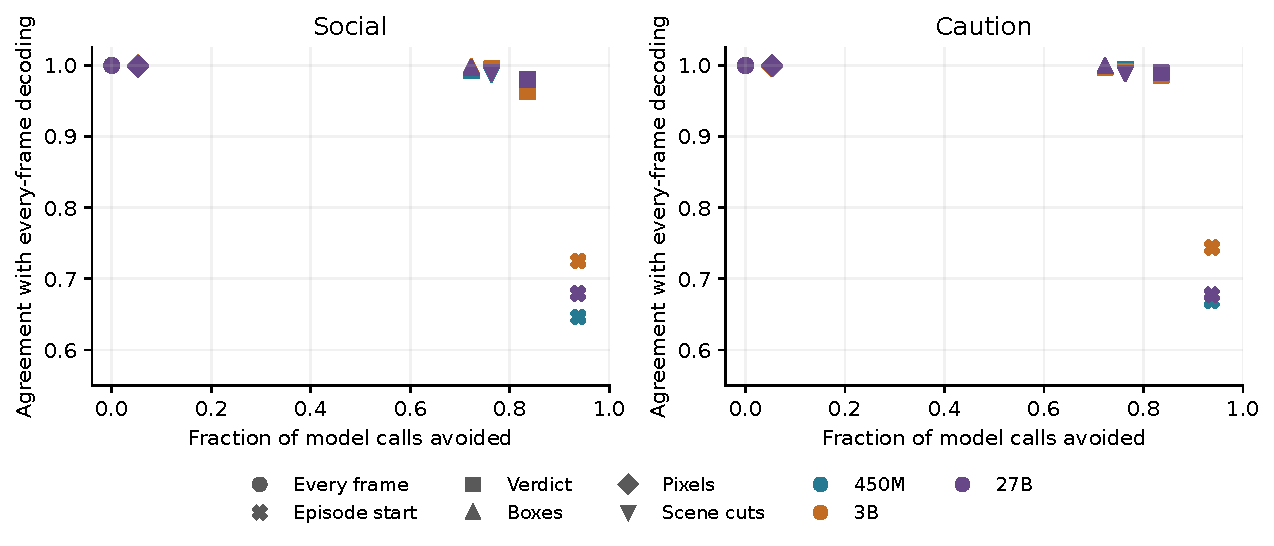
\includegraphics[width=.95\linewidth]{gating.pdf}
\caption{All six invocation policies, averaged over three seeds.
The fixed pixel threshold invokes on most jittered frames; the
verdict and box rules avoid more calls in this replay.
The figure does not compare tuned pixel gates or measured energy.}
\label{fig:gating}
\end{figure}

The 27B decode helper records a mean \DecodeSeconds{} seconds per
actual decode. This timing is specific to the GPU, cached
preprocessing, prompt, and short response used here. The experiment
does not measure complete system energy, detector-plus-host latency,
or production throughput. Detector work continues on skipped
frames. Multiplying avoided calls by this decode time is an
estimate of avoided model work, not an end-to-end saving measurement.
Likewise, the poor savings of this one pixel threshold under
deliberate pixel jitter do not establish that semantic gates are
always necessary.

\subsection{Delay includes unresolved cuts}
Time from a scene cut to the next invocation is not the same as
time to a necessary action correction: some scene changes require
no different action. Even as a descriptive responsiveness measure,
it must include cuts whose next invocation is not observed.

There are \PostCuts{} cuts after episode start. Under the verdict
gate, \ResolvedCuts{} have an observed later or same-step invocation,
and \CensoredCuts{} remain unresolved when the episode ends.
The observed delays have mean \ResolvedDelay{} steps and maximum
\MaxDelay{} steps; \SlowCuts{} exceed one step. The unresolved
cases are right-censored, not zero-delay successes. The historical
0.984-step average included the 60 zero-delay episode starts and
excluded unresolved cuts. It cannot support a one-frame response
claim. Table~\ref{tab:gate-controls} reports all gates using the
correct post-start denominator; the analysis also supplies each
cut's event or censoring record.

\section{Transfer to rendered scenes}
\subsection{Changing the visual domain}
We render paired present and absent scenes in MuJoCo
\citep{mujoco}. Each pair shares camera, room, and lighting draws.
The study first uses capsule-based human geometry, then one
textured human scan from Digital Reality Lab's HSRD-100 collection
\citep{hsrd}. Evaluation has 100 scene draws, each rendered with
and without the person. The human identity and pose are fixed;
rooms, camera placement, and illumination vary.

Two pixel versions survive in the records. Their scene draws are
identical, but their PNG hashes differ. The original LFM transfer
runs and the 3B training follow-ups use the first version; the 27B
runs and later 450M follow-ups use the second. We pair arms within
each run. The mixed-versus-fixed-baseline comparisons below use
identical pixels and mode checkpoints. Comparisons across pixel
versions cannot attribute every change to adapter training alone.
Host transfer tests use requested-mode packets as in the original
conditioning experiment; detector performance is evaluated separately.

All three YOLO sizes miss all 100 present capsule scenes at each
of the two tested capsule appearance settings. On the scan-based
scenes, the nano detector finds 99 of 100 present scenes with no
false alarms; the medium detector has no errors on this set.
The change establishes that this particular representation of the
person matters for these detectors. It does not separate all
effects of mesh geometry, texture, and rendering, or establish a
general simulator-to-real transfer result. Indeed, the tested
direction is photographs to rendered scenes.

A 3B diagnostic with direct caution text has a 0.267 difference
between present and absent stop shares on a 60-image capsule
subset. The source code uses the frozen host without an adapter
for that diagnostic Text arm, unlike the main Text control.
The result is partial discrimination, not evidence that every
host perceives the capsule reliably.

\subsection{Training domain and baseline choice}
We compare the original photograph-trained adapters with mixed
training on the 80 photographs plus 40 present and 40 absent
rendered training scenes. Rendered training uses a separate draw
seed and scene-index range. The doubled-budget mixed recipe uses
384 steps. Most follow-ups use all three seeds at 450M and 27B;
the 3B mixed variants have only seeds 42 and 1042. These are
targeted follow-ups, not a complete factorial design.

Table~\ref{tab:transfer} separates raw Packet behavior from the
constant baseline. In the mixed recipe, retraining the constant
adapter can make it strongly favor a person-directed action even
without mode input. A small Packet--Constant contrast can therefore
reflect a changed baseline, a weak mode adapter, or both.

The August 27 follow-up pairs the mixed mode adapter with the
original photograph-trained constant adapter. The Packet action
sequence stays the same; only the comparison baseline changes.
At 27B, the mean social and caution contrasts become 0.950 and
0.820 on rendered present scenes. Explore has a small contrast
because the original constant adapter already proceeds on most
rendered scenes. At 450M, the same analysis exposes a real explore
failure: Packet proceeds on only 0.167 of present scenes while
the original constant adapter proceeds on all of them. The original
constant weights are reused, but their Text control is evaluated
again. Across the two pixel versions, eight Text actions differ
in the 450M comparisons; the constant, Packet, and swapped-Packet
action sequences used for the fixed-baseline checks agree.

\begin{table}[htbp]\centering\small
\caption{Rendered present scenes (100 draws). Photo: original training;
Mixed: mixed-domain mode and constant adapters, 384 steps;
Mixed/fixed: the same mixed mode adapter with the original constant
baseline. The Packet column is unchanged between the two mixed rows.
Brackets give within-label scene-bootstrap intervals.}\label{tab:transfer}
\begin{tabular}{lllrrrl}\toprule
Host & Recipe & Mode & Seeds & Constant & Packet & Packet--Constant\\\midrule
450M & Photo & Social & 3 & 0.000 & 0.467 & 0.467 [0.373, 0.563] \\
450M & Photo & Caution & 3 & 0.000 & 0.690 & 0.690 [0.673, 0.707] \\
450M & Photo & Explore & 3 & 1.000 & 0.833 & -0.167 [-0.200, -0.133] \\
450M & Mixed & Social & 3 & 0.263 & 0.500 & 0.237 [0.137, 0.337] \\
450M & Mixed & Caution & 3 & 0.253 & 0.833 & 0.580 [0.517, 0.643] \\
450M & Mixed & Explore & 3 & 0.483 & 0.167 & -0.317 [-0.387, -0.250] \\
450M & Mixed/fixed & Social & 3 & 0.000 & 0.500 & 0.500 [0.400, 0.600] \\
450M & Mixed/fixed & Caution & 3 & 0.000 & 0.833 & 0.833 [0.800, 0.867] \\
450M & Mixed/fixed & Explore & 3 & 1.000 & 0.167 & -0.833 [-0.867, -0.800] \\
3B & Photo & Social & 3 & 0.000 & 0.060 & 0.060 [0.023, 0.103] \\
3B & Photo & Caution & 3 & 0.000 & 0.410 & 0.410 [0.383, 0.440] \\
3B & Photo & Explore & 3 & 1.000 & 1.000 & 0.000 [0.000, 0.000] \\
3B & Mixed & Social & 2 & 0.500 & 0.500 & 0.000 [-0.100, 0.100] \\
3B & Mixed & Caution & 2 & 0.070 & 1.000 & 0.930 [0.895, 0.960] \\
3B & Mixed & Explore & 2 & 0.430 & 1.000 & 0.570 [0.540, 0.605] \\
27B & Photo & Social & 3 & 0.030 & 0.623 & 0.593 [0.560, 0.623] \\
27B & Photo & Caution & 3 & 0.013 & 0.623 & 0.610 [0.547, 0.673] \\
27B & Photo & Explore & 3 & 0.957 & 1.000 & 0.043 [0.020, 0.067] \\
27B & Mixed & Social & 3 & 0.357 & 0.980 & 0.623 [0.583, 0.663] \\
27B & Mixed & Caution & 3 & 0.347 & 0.833 & 0.487 [0.440, 0.533] \\
27B & Mixed & Explore & 3 & 0.297 & 1.000 & 0.703 [0.660, 0.743] \\
27B & Mixed/fixed & Social & 3 & 0.030 & 0.980 & 0.950 [0.927, 0.973] \\
27B & Mixed/fixed & Caution & 3 & 0.013 & 0.833 & 0.820 [0.790, 0.853] \\
27B & Mixed/fixed & Explore & 3 & 0.957 & 1.000 & 0.043 [0.023, 0.067] \\

\bottomrule\end{tabular}
\end{table}

Some failures coincide exactly with held-out phrase assignment.
For the mixed 27B seed-42 caution adapter, the target-action shares
on rendered present scenes are 0.000 for phrase 8 and 1.000 for
phrase 9. At 450M, the mixed social adapter shows that same
0.000/1.000 split at all three seeds. The evaluation alternates
the phrases across scene IDs rather than applying both phrases
to every image, so this is a descriptive association. It is
strong evidence against assuming broad paraphrase robustness;
it does not by itself identify the causal contribution of
phrase and scene subset.

Crossing initialization and batch-order seeds in selected mixed
training runs changes both Packet and Constant behavior
(Table~\ref{tab:order}). At 450M, the weak caution Packet remains
at 0.500 with initialization 42 and order 1042, while initialization
1042 and order 42 reaches 1.000. At 27B, both crossed runs reach
1.000 on the photographic caution evaluation. These few
interventions narrow the failure cases. They do not justify a
general decomposition of initialization, optimization, and
model-size effects. The complete per-seed rendered results,
including the shorter mixed and doubled photo-only recipes,
appear in Appendix~\ref{app:transfer}.

\section{Limitations and implications}
The packet can carry an operator mode at 27B, and a small detector
can usefully decide when to request a new action in the tested
stream. Those conclusions survive the additional controls.
Their scope is a finite action task with known labels, fixed
prompts, a small number of adapter seeds, and reused image sets.

Several experiments are needed before making broader claims.
Unrestricted generation and instruction following need tasks
whose outputs are more than three action labels. Paraphrase
robustness needs additional phrases crossed with the same images,
rather than two phrases assigned to alternating subsets.
New image collections and new human identities would test
domain generalization. A live stream with task-relevant changes,
measured complete-system latency and energy, and an action-level
failure criterion would be required for deployment claims.
These are extensions of the present claims, not measurements
that this paper already supplies.

The comparisons also leave mechanisms unresolved. The main
Text arm uses a constant adapter; auxiliary losses and training
random draws differ between adapter types. The multi-scale
comparison changes model family as well as size. The box
projection and blank-image studies cover only the two LFM
hosts. Mixed-domain follow-ups were chosen after observing
failures and do not include every seed and recipe combination.
The bootstrap intervals cannot remove those design limitations.

For this architecture, the practical lessons are to report
raw action shares alongside baseline differences, verify
detector errors on the images where they occur, distinguish
agreement from correctness, and retain unresolved response
delays. Conditioning strength alone is not a safety mechanism.

\section{Reproducibility and evidence}
The public reproduction package contains \EvidenceFiles{} original
JSON records, the study-specific experiment harness, input and
checkpoint identities, CPU analysis, and this manuscript's
renderer:
\begin{center}
\url{https://github.com/kortexa-ai/legolm.paper/tree/main/reproductions/lookout-captain}
\end{center}
The analysis verifies evidence-file hashes, recomputes
\ScalarChecks{} reported scalar quantities from
\AuditedImageRecords{} individual-image result records, replays
their parsers, and evaluates 36 host/mode/gate combinations.
The latter contain repeated measurements of the same episodes,
not 36 independent datasets. Each table and figure is generated
from the checked analysis. Original readings remain available
alongside the corrected presentation.

The release distinguishes exact reproduction of saved-data
analysis from repetition of training and inference. All 72
referenced adapter, projection, classifier, and detector files
were found and matched their recorded SHA-256 identities in
the publication audit. The 27B host revision was recorded in
the experiment. The LFM records name models without immutable
revisions; the release pins the cached snapshots recovered
from the study machine and labels their provenance accordingly.
The original records also lack a complete environment lock
and hashes of any uncommitted source at execution time.
A pinned public harness and recovered checkpoints make the
study inspectable, but do not retroactively supply missing
historical provenance or promise bitwise retraining.

The original temporary rendered PNG files were not recovered.
The evaluation records retain the scene draws, image IDs, and
both sets of pixel hashes. Reproduction commands regenerate
the scenes and check those identities; a different rendering
device can produce a different pixel version. Saved-response
analysis requires neither these PNGs nor a GPU.

The HSRD-100 asset is attributed to Digital Reality Lab and
used under CC BY 4.0. The package identifies the exact archive
and its hash. External image, model, detector, and mesh
licenses remain with their respective sources.

\section{Conclusion}
Mode packets change action selection in frozen vision-language
models from 450M to 27B, with effects that depend on mode,
adapter seed, and instruction phrase. Detector-controlled
selection and event-triggered invocation can preserve much
of that behavior in a restricted replay while avoiding most
model calls. The same experiments reveal false actions,
phrase-specific failures, unstable baselines, and long or
unresolved invocation delays. Those observations define both
the demonstrated result and the work needed for a broader
multimodal or robotic system.

\FloatBarrier
\bibliographystyle{plainnat}
\bibliography{references}
\clearpage
\appendix
\section{Conditioning controls and seed variation}
\begin{table}[htbp]\centering\small
\caption{Wrong-mode control, absent-image target-action share, and
per-seed Packet--Constant contrasts. Seed order is 42, 1042, 2042.
For explore, the absent target action is proceed and a share of one
is correct. For social and caution, a nonzero absent share is an
incorrect greet or stop.}\label{tab:controls}
\begin{tabular}{lllll}\toprule
Host & Mode & Packet--Swapped & Packet on absent & Per-seed Packet--Constant\\\midrule
450M & Social & 0.633 [0.500, 0.767] & 0.011 [0.000, 0.033] & 0.133/0.667/0.200 \\
450M & Caution & 0.678 [0.556, 0.800] & 0.033 [0.000, 0.078] & 0.967/0.400/0.967 \\
450M & Explore & 0.522 [0.456, 0.589] & 1.000 [1.000, 1.000] & -0.033/0.333/-0.167 \\
3B & Social & 0.489 [0.322, 0.667] & 0.044 [0.011, 0.089] & 0.133/-0.233/0.167 \\
3B & Caution & 0.756 [0.711, 0.811] & 0.022 [0.000, 0.056] & 0.133/0.900/0.967 \\
3B & Explore & 0.800 [0.722, 0.867] & 1.000 [1.000, 1.000] & 0.500/0.833/0.333 \\
27B & Social & 0.978 [0.944, 1.000] & 0.000 [0.000, 0.000] & 0.433/0.533/0.967 \\
27B & Caution & 1.000 [1.000, 1.000] & 0.044 [0.011, 0.089] & 0.767/0.833/1.000 \\
27B & Explore & 0.989 [0.967, 1.000] & 1.000 [1.000, 1.000] & 0.800/0.600/0.000 \\

\bottomrule\end{tabular}
\end{table}

\section{Contrary text and box controls}
\begin{table}[htbp]\centering\footnotesize
\caption{Contrary-text comparisons on the initial 30 present and
30 absent photographs, averaged over three seeds. $P$: Packet;
$T^-$: contrary text with the constant adapter. The paired
difference is measured on present images. Absent $P$ is a
false action for social/caution and correct proceed for explore.}
\label{tab:conflict}
\begin{tabular}{lllrrrlr}\toprule
Host & Mode & Dose & $P$ & $T^-$ & $P+T^-$ &
$(P+T^-)-T^-$ & Absent $P$\\\midrule
450M & Social & 0.15 & 0.633 & 0.289 & 0.556 & 0.267 [0.067, 0.467] & 0.011 \\
450M & Caution & 0.15 & 1.000 & 0.178 & 0.989 & 0.811 [0.722, 0.889] & 0.033 \\
450M & Explore & 0.15 & 0.522 & 0.022 & 0.333 & 0.311 [0.222, 0.400] & 1.000 \\
450M & Social & 0.225 & 0.500 & 0.111 & 0.489 & 0.378 [0.167, 0.589] & 0.033 \\
450M & Caution & 0.225 & 1.000 & 0.267 & 1.000 & 0.733 [0.689, 0.789] & 0.078 \\
450M & Explore & 0.225 & 0.467 & 0.467 & 0.489 & 0.022 [-0.122, 0.167] & 1.000 \\
3B & Social & 0.15 & 0.489 & 0.033 & 0.278 & 0.244 [0.133, 0.367] & 0.044 \\
3B & Caution & 0.15 & 0.756 & 0.000 & 0.411 & 0.411 [0.322, 0.500] & 0.022 \\
3B & Explore & 0.15 & 1.000 & 0.056 & 0.922 & 0.867 [0.778, 0.944] & 1.000 \\
3B & Social & 0.225 & 0.478 & 0.644 & 0.500 & -0.144 [-0.344, 0.056] & 0.133 \\
3B & Caution & 0.225 & 0.889 & 0.011 & 0.744 & 0.733 [0.678, 0.789] & 0.178 \\
3B & Explore & 0.225 & 1.000 & 0.011 & 1.000 & 0.989 [0.967, 1.000] & 1.000 \\
27B & Social & 0.15 & 0.978 & 0.222 & 0.767 & 0.544 [0.456, 0.644] & 0.000 \\
27B & Caution & 0.15 & 1.000 & 0.111 & 0.889 & 0.778 [0.711, 0.844] & 0.044 \\
27B & Explore & 0.15 & 1.000 & 0.289 & 0.978 & 0.689 [0.600, 0.778] & 1.000 \\
27B & Social & 0.225 & 0.989 & 0.333 & 0.889 & 0.556 [0.467, 0.644] & 0.000 \\
27B & Caution & 0.225 & 1.000 & 0.022 & 0.911 & 0.889 [0.833, 0.944] & 0.033 \\
27B & Explore & 0.225 & 1.000 & 0.622 & 1.000 & 0.378 [0.300, 0.456] & 1.000 \\

\bottomrule\end{tabular}
\end{table}

\begin{table}[htbp]\centering\small
\caption{Projection experiments on the 100 present photographs.
Means use three seeds. Blank replaces the host image at
projection training and evaluation; the detector still sees
the photograph. Lying supplies zeros on present photographs.
The full records also contain absent-image false-box responses.}
\label{tab:boxes}
\begin{tabular}{lllrrrl}\toprule
Host image & Host & Mode & Switch & Boxes & Lying & Boxes--Switch\\\midrule
Visible & 450M & Social & 0.590 & 0.533 & 0.537 & -0.057 [-0.100, -0.010] \\
Visible & 450M & Caution & 0.930 & 0.923 & 0.967 & -0.007 [-0.050, 0.040] \\
Visible & 3B & Social & 0.443 & 0.453 & 0.457 & 0.010 [-0.010, 0.033] \\
Visible & 3B & Caution & 0.703 & 0.927 & 0.760 & 0.223 [0.187, 0.260] \\
Blank & 450M & Social & 0.000 & 0.087 & 0.000 & 0.087 [0.060, 0.117] \\
Blank & 450M & Caution & 0.000 & 0.160 & 0.000 & 0.160 [0.127, 0.193] \\
Blank & 3B & Social & 0.000 & 0.000 & 0.000 & 0.000 [0.000, 0.000] \\
Blank & 3B & Caution & 0.317 & 0.333 & 0.333 & 0.017 [0.003, 0.033] \\

\bottomrule\end{tabular}
\end{table}

\section{Invocation controls and censoring}
\begin{table}[htbp]\centering\small
\caption{27B gate controls. Agreement is averaged across three
seeds. Wakes/cuts counts only the 167 post-start cuts with an
observed next invocation; mean delay excludes censored cases
and must be read alongside their count. Gate schedules are
identical across hosts and seeds.}\label{tab:gate-controls}
\begin{tabular}{lrrrlrr}\toprule
Gate & Calls avoided & Caution agree & Social agree &
Resolved cuts & Mean delay & Censored\\\midrule
Every frame & 0.000 & 1.000 & 1.000 & 167/167 & 0.00 & 0 \\
Episode start & 0.938 & 0.677 & 0.679 & 0/167 & -- & 167 \\
Verdict & 0.835 & 0.990 & 0.981 & 130/167 & 1.44 & 37 \\
Boxes & 0.723 & 1.000 & 0.997 & 148/167 & 0.42 & 19 \\
Pixels & 0.053 & 1.000 & 0.999 & 167/167 & 0.00 & 0 \\
Scene cuts & 0.764 & 0.989 & 0.990 & 167/167 & 0.00 & 0 \\

\bottomrule\end{tabular}
\end{table}

The historical lag records are preserved. The corrected analysis
reconstructs cut-to-next-invocation events directly from the step
logs. If several cuts precede a single invocation, each cut
receives its own delay. A cut on the last step without an
invocation is censored at duration zero. Such a record does not
mean the model responded immediately. A descriptive survival
curve is included in the machine-readable analysis; cuts within
an episode are dependent, so it is not used as an independent
population-level survival test.

\section{Training-order diagnostics}
\begin{table}[htbp]\centering\small
\caption{Caution on the 30 present photographic images under
mixed training at 384 steps. Initialization and training-order
seeds are crossed only in these selected runs. Both mode and
constant adapters are retrained in each row.}\label{tab:order}
\begin{tabular}{lrrrr}\toprule
Host & Initialization & Order & Constant & Packet\\\midrule
450M & 42 & 42 & 0.567 & 0.500 \\
450M & 1042 & 1042 & 0.167 & 0.967 \\
450M & 42 & 1042 & 0.200 & 0.500 \\
450M & 1042 & 42 & 0.767 & 1.000 \\
27B & 42 & 42 & 0.467 & 0.500 \\
27B & 1042 & 1042 & 0.533 & 1.000 \\
27B & 42 & 1042 & 0.233 & 1.000 \\
27B & 1042 & 42 & 0.433 & 1.000 \\

\bottomrule\end{tabular}
\end{table}

\section{Complete rendered-scene seed results}\label{app:transfer}
Each row below uses the same 100 present rendered scene draws.
The recipe identifiers match the artifact filenames after
\texttt{vision-mode-r3b-}. A bare host uses the original
photographic adapters. \texttt{x2door} doubles photographic
training to 384 steps; \texttt{mxdoor} adds rendered training
at 192 steps; \texttt{mx2door} uses mixed training at 384 steps;
\texttt{mx2ndoor} retains that mode adapter but uses the original
constant baseline. \texttt{mx2o1042door} and
\texttt{mx2o42door} change the training-order seed. Slashes
separate results in the listed seed order.

\small
\begin{longtable}{lll>{\raggedright\arraybackslash}p{1.46in}>{\raggedright\arraybackslash}p{1.46in}}
\caption{Per-seed rendered Packet shares and baseline contrasts.}\\
\toprule
Recipe--host & Mode & Seeds & Packet & Packet--Constant\\\midrule
\endfirsthead
\toprule Recipe--host & Mode & Seeds & Packet & Packet--Constant\\\midrule
\endhead
27b & Social & 42,1042,2042 & 0.930/0.940/0.000 & 0.840/0.940/0.000 \\
27b & Caution & 42,1042,2042 & 0.550/0.820/0.500 & 0.520/0.810/0.500 \\
27b & Explore & 42,1042,2042 & 1.000/1.000/1.000 & 0.120/0.010/0.000 \\
3b & Social & 42,1042,2042 & 0.020/0.080/0.080 & 0.020/0.080/0.080 \\
3b & Caution & 42,1042,2042 & 0.000/0.230/1.000 & 0.000/0.230/1.000 \\
3b & Explore & 42,1042,2042 & 1.000/1.000/1.000 & 0.000/0.000/0.000 \\
450m & Social & 42,1042,2042 & 0.500/0.410/0.490 & 0.500/0.410/0.490 \\
450m & Caution & 42,1042,2042 & 1.000/0.070/1.000 & 1.000/0.070/1.000 \\
450m & Explore & 42,1042,2042 & 1.000/1.000/0.500 & 0.000/0.000/-0.500 \\
mx2door-27b & Social & 42,1042,2042 & 1.000/1.000/0.940 & 0.790/0.150/0.930 \\
mx2door-27b & Caution & 42,1042,2042 & 0.500/1.000/1.000 & 0.430/0.970/0.060 \\
mx2door-27b & Explore & 42,1042,2042 & 1.000/1.000/1.000 & 0.280/0.880/0.950 \\
mx2door-3b & Social & 42,1042 & 0.500/0.500 & 0.500/-0.500 \\
mx2door-3b & Caution & 42,1042 & 1.000/1.000 & 0.860/1.000 \\
mx2door-3b & Explore & 42,1042 & 1.000/1.000 & 0.140/1.000 \\
mx2door-450m & Social & 42,1042,2042 & 0.500/0.500/0.500 & 0.500/-0.290/0.500 \\
mx2door-450m & Caution & 42,1042,2042 & 0.500/1.000/1.000 & 0.360/0.940/0.440 \\
mx2door-450m & Explore & 42,1042,2042 & 0.000/0.000/0.500 & -0.860/-0.150/0.060 \\
mx2ndoor-27b & Social & 42,1042,2042 & 1.000/1.000/0.940 & 0.910/1.000/0.940 \\
mx2ndoor-27b & Caution & 42,1042,2042 & 0.500/1.000/1.000 & 0.470/0.990/1.000 \\
mx2ndoor-27b & Explore & 42,1042,2042 & 1.000/1.000/1.000 & 0.120/0.010/0.000 \\
mx2ndoor-450m & Social & 42,1042,2042 & 0.500/0.500/0.500 & 0.500/0.500/0.500 \\
mx2ndoor-450m & Caution & 42,1042,2042 & 0.500/1.000/1.000 & 0.500/1.000/1.000 \\
mx2ndoor-450m & Explore & 42,1042,2042 & 0.000/0.000/0.500 & -1.000/-1.000/-0.500 \\
mx2o1042door-27b & Social & 42 & 1.000 & 0.230 \\
mx2o1042door-27b & Caution & 42 & 1.000 & 0.990 \\
mx2o1042door-27b & Explore & 42 & 1.000 & 0.780 \\
mx2o1042door-450m & Social & 42 & 0.500 & -0.350 \\
mx2o1042door-450m & Caution & 42 & 0.500 & 0.410 \\
mx2o1042door-450m & Explore & 42 & 0.500 & 0.440 \\
mx2o42door-27b & Social & 1042 & 1.000 & 1.000 \\
mx2o42door-27b & Caution & 1042 & 1.000 & 0.980 \\
mx2o42door-27b & Explore & 1042 & 1.000 & 0.020 \\
mx2o42door-450m & Social & 1042 & 0.500 & 0.500 \\
mx2o42door-450m & Caution & 1042 & 1.000 & 0.010 \\
mx2o42door-450m & Explore & 1042 & 0.490 & 0.480 \\
mxdoor-3b & Social & 42,1042 & 0.500/0.430 & 0.480/-0.430 \\
mxdoor-3b & Caution & 42,1042 & 1.000/1.000 & 0.950/0.860 \\
mxdoor-3b & Explore & 42,1042 & 1.000/1.000 & 0.070/1.000 \\
mxdoor-450m & Social & 42,1042,2042 & 0.500/0.500/0.500 & 0.140/0.290/0.500 \\
mxdoor-450m & Caution & 42,1042,2042 & 0.500/1.000/1.000 & 0.160/0.210/0.360 \\
mxdoor-450m & Explore & 42,1042,2042 & 0.000/0.060/0.500 & -0.300/0.060/0.140 \\
x2door-3b & Social & 42,1042 & 0.030/0.020 & 0.030/0.020 \\
x2door-3b & Caution & 42,1042 & 0.310/0.180 & 0.310/0.180 \\
x2door-3b & Explore & 42,1042 & 1.000/1.000 & 0.000/0.000 \\

\bottomrule
\end{longtable}
\normalsize
\end{document}
